% The LaTeX is in here!
\documentclass{article}
\usepackage{graphicx}
\usepackage{parskip}
\usepackage{float}
\usepackage{hyperref}
\usepackage[utf8]{inputenc}
\setlength{\parindent}{4em}
% \renewcommand{\baselinestretch}{2.0}
\usepackage[english]{babel}
\graphicspath{ {images/} }

\begin{document}
    \begin{center}
    
\includegraphics[scale=0.5]{unb}
    \vspace{15mm}
    \textbf{Universidade de Brasília - UnB}\\
    \textbf{Instituto de Exatas}\\
    \textbf{Departamento de Ciência da Computação}\\
    \vspace{15mm}
    \textbf{Rodrigo Chaves - 13/0132624}\\
    \textbf{Gabriel Mesquita - 13/0024242}\\
    \vspace{15mm}
    \textbf{Test-drive Development}\\
    \vspace{15mm}
    \textbf{Brasília - DF}\\
    \textbf{2016}
  \end{center}

  \clearpage

  \begin{center}
    Gabriel Mesquita ...\\
    Rodrigo de Araujo Chaves\\
    \vspace{30mm}
    \textbf{Test-driven Development}
    \vspace{30mm}
    \begin{flushright}
      Dissertação sobre por que Test-driven development\\
      é pratica que melhorar a qualidade\\
      final do software apresentanda à disciplina\\
      de Engenharia de Software da Universidade de Brasília.\\
    \end{flushright}
    \vspace{60mm}
    \textbf{Brasília - DF}\\
    \textbf{2016}
  \end{center}

  \clearpage

  \section{Introdução}

  \section{O que é Test-driven Development}

  Test-driven development é um prática de desenvolvimento de software que tem 
  sido usada esporádicamente por decadas. Com essa pratica, um engenheiro de 
  software passo por ciclos entre escrever um teste de unidade que falha e 
  escrevendo a implementação do software para passar nesses testes. 
  Test-driven development tem recentemente resurgindo como uma pratica critica 
  possibilitando metodologias de desenvolvimento ágil de software.

  Quando discutimos sobre TDD, é considerado um conjunto de tarefas requiridas 
  que podem ser implementadas em poucos dias ou menos. Na imagem 1, engenheiros 
  de software produzem código de produção através de rápidas interações como as 
  que seguem:

  \begin{enumerate}
    \item O primeiro passo é adicionar um teste simples o qual é suficiente 
    para a suíte de teste falhar.
    \item Depois executamos nossa suíte para confirmar que os testes realmente 
    estão falhando.
    \item Agora atualize-se o código funcional afim de passar no novo teste.
    \item Executamos a suíte de teste para verificarmos se agora realmente 
    passarmos no novo teste.
    \item Agora com o teste passando: são removidos as duplicações de código 
    afim de limpar o código.
  \end{enumerate}

  \begin{figure}[H]
    \centering
    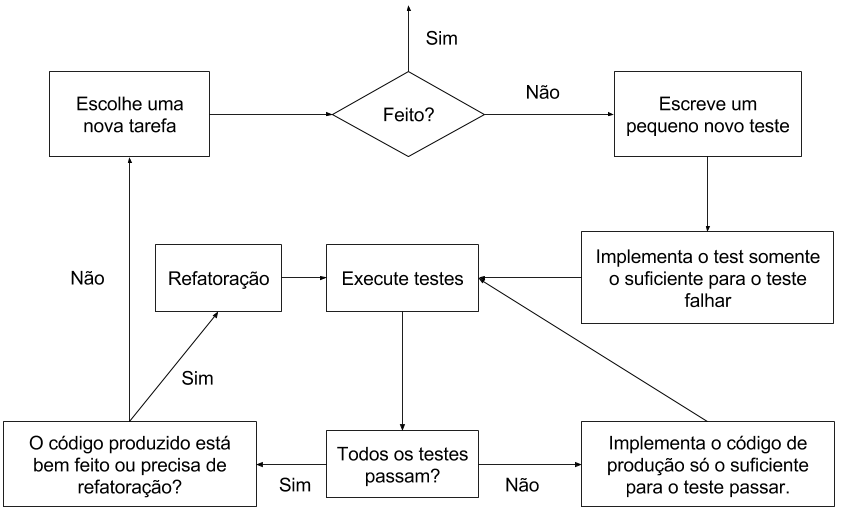
\includegraphics[scale=0.4]{tdd}
    \caption{Fluxograma do TDD}
  \end{figure}

  \section{Referências}

  Nachiappan Nagappan, E. Michael Maximilien, Thirumalesh Bhat,
  Laurie Williams, Realizing quality improvement through test driven 
  development: results and experiences of four industrial teams. Disponível em
  \url{http://link.springer.com/article/10.1007/s10664-008-9062-z#/page-1}.
  Acessado em 26 de maio de 2016.

  Andreas Augustin, Test-Driven Development: Concepts, Taxonomy, and Future 
  Direction. Disponível em \url{https://www.semanticscholar.org/paper/Test-
  Driven-Development-Concepts-Taxonomy-and-Janzen-Saiedian/bdcd570eb6a45d7a
  9107a18e25f54b741b92177f/pdf}. Acessado em 26 de maio de 2016

\end{document}